%%%%%%%% MICE: Mixture of In-Context Experts for recurring concept drift. ICML template (icml2026.sty until the
%%%%%%%% 2027 style is released). Full draft of 2026-10-05. Every number is taken from logs/EXPERIMENT_LOG.md and
%%%%%%%% results_paper/ (code/make_paper_tables.py); tab_*_rows.tex are generated, do not edit them by hand.
%%%%%%%% The skeleton of 2026-10-03 is kept in old/main_skeleton_1003.tex.
\documentclass{article}

\usepackage{microtype}
\usepackage{graphicx}
\usepackage{booktabs}
\usepackage{hyperref}
\newcommand{\theHalgorithm}{\arabic{algorithm}}

\usepackage{icml2026}          % blind review
% \usepackage[accepted]{icml2026}

\usepackage{amsmath}
\usepackage{amssymb}
\usepackage{mathtools}
\usepackage{amsthm}
\usepackage[capitalize,noabbrev]{cleveref}
\usepackage{algorithm}
\usepackage{algorithmic}
\usepackage[textsize=tiny]{todonotes}
\usepackage{tikz}

\theoremstyle{plain}
\newtheorem{theorem}{Theorem}
\newtheorem{proposition}{Proposition}
\newtheorem{lemma}{Lemma}
\newtheorem{corollary}{Corollary}
\theoremstyle{definition}
\newtheorem{definition}{Definition}
\newtheorem{assumption}{Assumption}
\newtheorem{observation}{Observation}
\theoremstyle{remark}
\newtheorem{remark}{Remark}

% Shared notation. Vectors bold (\mathbf), matrices calligraphic (\mathcal), names and operators upright.
\newcommand{\vx}{\mathbf{x}}
\newcommand{\vX}{\mathbf{X}}
\newcommand{\vz}{\mathbf{z}}
\newcommand{\vZ}{\mathbf{Z}}
\newcommand{\vw}{\mathbf{w}}
\newcommand{\valpha}{\boldsymbol{\alpha}}
\newcommand{\cC}{\mathcal{C}}      % context (a set of labelled rows)
\newcommand{\cY}{\mathcal{Y}}      % label set
\newcommand{\cH}{\mathcal{H}}      % hypothesis space
\newcommand{\cD}{\mathcal{D}}
\newcommand{\cS}{\mathcal{S}}      % data stream
\newcommand{\E}{\mathbb{E}}
\newcommand{\R}{\mathbb{R}}
\newcommand{\Prob}{\Pr}
\newcommand{\KL}{\mathrm{KL}}
\newcommand{\Regret}{\mathrm{Regret}}
\newcommand{\Div}{\mathrm{D}}
\DeclareMathOperator*{\argmin}{arg\,min}
\DeclareMathOperator*{\argmax}{arg\,max}
\DeclareMathOperator{\AUROC}{AUROC}

\crefname{assumption}{Assumption}{Assumptions}
\crefname{observation}{Observation}{Observations}
\crefname{appendix}{Appendix}{Appendices}
\newcommand{\method}{\textsc{MICE}}   % Mixture of In-Context Experts
\makeatletter\newcommand{\rowinput}[1]{\@@input #1 }\makeatother   % expandable \input for generated table rows

\begin{document}

\twocolumn[
  \icmltitle{Recall or Relearn? A Mixture of In-Context Experts for Recurring Concept Drift}
  \icmlsetsymbol{equal}{*}
  \begin{icmlauthorlist}
    \icmlauthor{Anonymous Author(s)}{anon}
  \end{icmlauthorlist}
  \icmlaffiliation{anon}{Anonymous Institution}
  \icmlcorrespondingauthor{Anonymous Author(s)}{anon@anon.org}
  \icmlkeywords{concept drift, recurring concepts, tabular foundation models, in-context learning, online learning}
  \vskip 0.3in
]
\printAffiliationsAndNotice{}

\begin{abstract}
Tabular foundation models (TFMs) learn a data stream through their context, so a past concept can be recalled by
putting its rows back into the context, at no training cost. Current in-context stream learners do not use this:
a sliding context forgets a concept once it leaves the window, and a detector that resets the context is unsafe,
losing up to 9.6 points to a plain window on real streams. We ask when recalling a concept is worth more than
relearning it, and how to recall without paying when there is nothing to recall. We show that the value of memory is
set by the TFM's learning curve: the gain of recall over relearning is the area between the learning curve and the
accuracy of the stored context. We propose \method{}, a mixture of in-context experts, fast windows and stored
contexts, under a meta expert with two time scales. The fast level identifies a recurring concept within one batch
when the experts are separated by a margin; the slow level has a discounted regret of at most $\ln K/\eta$ against
the plain window at any time, with no assumption on the stream. On a pre-registered grid of recurring concepts, the
gain predicted from learning curves measured beforehand ranks the observed gains with Spearman 0.94, and \method{}
exceeds a reset detector on every stream with hard concepts, by 8.5 points on the hardest cell, and a sliding
window by 24 points on average. On 29 real streams \method{} is more accurate than all four in-context baselines on
23 and never more than 0.25 points below the plain window; a pre-registered test on six held-out segments confirms
both.
\end{abstract}

% =====================================================================================================
\section{Introduction}
\label{sec:intro}

A data stream revisits its past: seasons, weekdays, market regimes and sensor modes return. A learner that kept what
it knew about a concept can use it again when the concept recurs \citep{gama2014survey,lu2019learning}. For a
trained model this means keeping a pool of models and deciding which one to reuse
\citep{goncalves2013rcd,gama2014recurrent,zhao2025mooe}. Tabular foundation models (TFMs) such as TabPFN
\citep{hollmann2025tabpfn} and TabICL \citep{qu2025tabicl} change the cost of this idea. A TFM approximates posterior
prediction in one forward pass given a context of labelled rows \citep{muller2022pfn,nagler2023statistical}; its
knowledge of a concept \emph{is} a set of rows, and recalling the concept means conditioning on them. Memory needs no
training.

TFMs have already replaced incremental trees as stream learners: with a sliding memory they outperform adaptive tree
ensembles on non-stationary benchmarks \citep{lourenco2026streams}, and a prior with drifting causal models improves
them under temporal shift \citep{helli2024drift}. Neither line uses the free memory. A sliding context forgets a
concept once it leaves the window, and a drift-extrapolating prior models a trend rather than a return. Three
observations show what an in-context stream learner is missing, and what a remedy has to respect.

\begin{observation}[Sliding contexts forget]\label{obs:forget}
In the five batches after a concept recurs, a TFM with a FIFO context or with the dual memory of
\citet{lourenco2026streams} reaches 0.17, 0.39 and 0.51 accuracy on Sine, Stagger and Agrawal streams, whereas the
same TFM conditioned on the past rows of the recurring concept reaches at least 0.99; in steady state all contexts
are equally accurate.
\end{observation}

\begin{observation}[Relearning in context is cheap, for simple concepts]\label{obs:relearn}
A TFM relearns the concepts of the standard drift generators within about 200 rows, so resetting the context when a
drift detector fires \citep{gama2004ddm} already closes most of the gap of \cref{obs:forget} (0.81--0.88 in the same
five batches). Memory pays only for concepts that take many rows to learn: on mixtures with 100 centroids the TFM
needs more than 1000 rows to approach its asymptote.
\end{observation}

\begin{observation}[Resetting is unsafe]\label{obs:reset}
On 29 real streams the same reset detector is on average 1.8 points \emph{below} the plain FIFO context and up to 9.6
points below it: most rises of the error rate on real streams do not mean that the context has become useless.
\end{observation}

These observations raise the question of this paper: \emph{when should an in-context learner recall a past concept
rather than relearn it, and how can it do so without paying when there is nothing to recall?}

\textbf{Approach.} We treat every past context as an offline expert and the current window as an online expert, and
combine them with a meta expert, following the mixture of online and offline experts (MOOE) of
\citet{zhao2025mooe}. An in-context expert costs no training, which changes both the method and its analysis.
(i)~Which segments belong to the same concept is decided by a model-oriented discrepancy in the sense of
R-divergence \citep{zhao2023rdiv}; we show that the original form is blind to concepts that contradict each other on
the same inputs, which is the defining case of recurring drift, and that an excess-risk form repairs it.
(ii)~The meta expert has two time scales. A fast level restarts every batch and identifies a recurring concept in
one batch under a margin; a slow level decides whether following the fast level is worth it at all, with a
worst-case guarantee against the plain window. (iii)~The gain of recall over relearning then has a closed form in
the TFM's learning curve, so the value of memory can be measured before deployment.

\textbf{Contributions.}
\textbf{(1) Problem.} Recurring concept drift for in-context learners, where past contexts are free experts
(\cref{def:recur}), with three observations on forgetting, relearning and resetting.
\textbf{(2) Theory.} The blind spot of R-divergence under conflicting concepts and its excess-risk repair
(\cref{prop:blind}); identification in one batch under a margin (\cref{prop:block}); the recall-versus-relearn
formula (\cref{prop:recall}); and an any-time discounted regret bound for the slow level (\cref{prop:outer}).
\textbf{(3) Method.} \method{}, a training-free mixture of window and stored in-context experts whose every
component corresponds to one of these results.
\textbf{(4) Evidence.} Pre-registered tests on a controlled grid, where the learning curve predicts the gain of
memory and \method{} exceeds reset detection, window ensembles, incremental learners and trained MOOE; and 29 real
streams, where \method{} is the most accurate in-context policy on 23 and stays within 0.25 points of the plain
window on all.

% =====================================================================================================
\section{Recurring Concept Drift for In-Context Learners}
\label{sec:def}

\textbf{Setting.} A stream delivers batches of $B$ rows; the labels of a batch arrive one batch late. A frozen TFM
$f_\Theta(\cdot\mid\vx;\cC)$ predicts every batch from a context $\cC$ of at most $M$ labelled rows, and a
\emph{context policy} decides which rows form the context. The stream is a sequence of intervals $I_1,I_2,\dots$ with
distributions $P_1,P_2,\dots$ over $(\vx,y)$; concept drift occurs between intervals in the sense of
\citet{lu2019learning}.

\begin{definition}[Recurring in-context concept drift]\label{def:recur}
Let $\cC_k$ be a context of rows of interval $I_k$ and $f_\Theta(\cdot\,;\cC_k)$ the $k$-th \emph{in-context expert}.
The drift into interval $I_{K+1}$ is \emph{recurring} if $\min_{k\le K}\Div_T(P_{K+1}\,|\,P_k)\le\delta$, where
$\Div_T(Q\,|\,P)$ is the risk on $Q$ of the expert of $P$ minus that of the expert of $Q$ (\cref{def:excess}), and
\emph{new} otherwise.
\end{definition}

The definition is model-oriented: a drift is recurring when some stored context serves the new interval as well as
its own rows would. Three policies are the reference points of this paper. \emph{FIFO} is the plain sliding window: the context is the last $M$ labelled rows, first in, first out. It is the
simplest context policy and the building block of the short- and long-term memory of \citet{lourenco2026streams}. \emph{Reset} empties the context when the drift detection method (DDM) of
\citet{gama2004ddm} fires. \emph{Window ensemble} mixes FIFO contexts of several lengths. None of them has memory.

% =====================================================================================================
\section{Theory: From a Model-Oriented Discrepancy to Recall versus Relearn}
\label{sec:theory}

The analysis has four steps, one per component of the method: which contexts share a concept
(\cref{sec:th-disc}), how fast a recurring concept is identified (\cref{sec:th-fast}), what recalling it is worth
(\cref{sec:th-recall}), and what following the mixture can cost when nothing recurs (\cref{sec:th-slow}). All proofs
are in \cref{app:proofs}.

\textbf{Notation.} For a concept $P$ over $(\vx,y)$ and a loss $\ell$, the \emph{risk} of a context $\cC$ is
\[
  \epsilon_P(\cC)=\E_{(\vx,y)\sim P}\,\ell\bigl(f_\Theta(\cdot\mid\vx;\cC),y\bigr),
\]
and the \emph{learning curve} of $P$ is $R_P(n)=\E_{\cC\sim P^n}\,\epsilon_P(\cC)$. We write $p_\vx=P(\cdot\mid\vx)$
for the conditional, $P_X$ for the marginal, $H$ for the entropy and $\mathrm{JS}$ for the Jensen--Shannon
divergence.

\subsection{Which Contexts Share a Concept}
\label{sec:th-disc}

R-divergence \citep{zhao2023rdiv} declares two distributions identical \emph{for a model} when the hypothesis learned
on their mixture has the same risk on both. For an in-context learner that hypothesis is the TFM conditioned on the
union of the two contexts:
\begin{equation}\label{eq:rdiv}
  \Div_R(P\|Q)=\bigl|\epsilon_P(\cC_P\cup\cC_Q)-\epsilon_Q(\cC_P\cup\cC_Q)\bigr| .
\end{equation}
Its population behaviour follows from the principle behind prior-fitted networks, which approximate the posterior
predictive distribution \citep{muller2022pfn,nagler2023statistical}.

\begin{assumption}[Posterior-predictive limit]\label{ass:ppd}
With a context from $P$ alone, the TFM predicts the conditional $p_\vx$; with contexts of equal size from $P$ and
$Q$, it predicts the conditional of the mixture $U=\tfrac12(P+Q)$,
\[
  u_\vx=\alpha(\vx)\,p_\vx+\bigl(1-\alpha(\vx)\bigr)\,q_\vx,\qquad \alpha=\frac{P_X}{P_X+Q_X}.
\]
We denote the two predictors by $h_P$ and $h_U$.
\end{assumption}

\begin{definition}[Recall regret and excess-risk discrepancy]\label{def:excess}
For two concepts $P$ and $Q$, the \emph{recall regret} of $P$ on $Q$ is the risk that the context of $P$ incurs on
$Q$ beyond that of the context of $Q$ itself, and the \emph{excess-risk discrepancy} is the mean risk that pooling
the two contexts adds to each concept:
\begin{align}
  \Div_T(Q\,|\,P) &= \epsilon_Q(h_P)-\epsilon_Q(h_Q), \label{eq:transfer}\\
  \Div_E(P,Q) &= \tfrac12\bigl[\epsilon_P(h_U)-\epsilon_P(h_P)\bigr] \notag\\
              &\quad+\tfrac12\bigl[\epsilon_Q(h_U)-\epsilon_Q(h_Q)\bigr].
  \label{eq:excess}
\end{align}
\end{definition}

\begin{proposition}[Blind spot of R-divergence and its repair]\label{prop:blind}
Let \cref{ass:ppd} hold and let $\ell$ be the log-loss.
\begin{enumerate}
  \item[(i)] \emph{Decomposition.} The excess-risk discrepancy is the part of the divergence between the joints
  that covariate shift does not explain:
  \[
    \Div_E(P,Q)=\mathrm{JS}(P,Q)-\mathrm{JS}(P_X,Q_X)\;\ge\;0 .
  \]
  If $P_X=Q_X$, then $\Div_E(P,Q)=\E_{\vx}\,\mathrm{JS}(p_\vx,q_\vx)$, which is zero if and only if $p_\vx=q_\vx$
  almost surely.
  \item[(ii)] \emph{Blind spot.} Let $P_X=Q_X$ and let both concepts be deterministic, $y=g_P(\vx)$ and
  $y=g_Q(\vx)$, with disagreement mass $\rho=\Pr_{\vx}[g_P(\vx)\neq g_Q(\vx)]$. Then, for every $\rho\in[0,1]$,
  \[
    \Div_R(P\|Q)=0\qquad\text{whereas}\qquad \Div_E(P,Q)=\rho\ln2 .
  \]
  \item[(iii)] \emph{0-1 loss.} In the setting of (ii) with the 0-1 loss, $\Div_R(P\|Q)=0$ and
  $\Div_T(Q\,|\,P)=\rho$.
\end{enumerate}
\end{proposition}

\begin{remark}\label{rem:merge}
R-divergence asks whether the mixture hypothesis treats the two sets \emph{equally}. Two concepts that contradict
each other on the same inputs are treated equally badly, so the answer is yes although neither context helps the
other; this is the defining case of recurring drift. The excess-risk form asks whether pooling \emph{costs}
anything. With finite contexts it has a second term: if $P=Q$, pooling doubles the context and changes the risk by
$R_P(2n)-R_P(n)\le0$. The empirical excess is interference minus pooling gain, so merging two contexts when it is at
most $\delta$ merges exactly when pooling helps more than the concepts interfere. \method{} uses the directed form
\eqref{eq:transfer} as its merge statistic, which is also the regret that recalling the stored expert would incur
(\cref{def:recur}).
\end{remark}

\subsection{The Fast Level: Identification under a Margin}
\label{sec:th-fast}

Following \citet{zhao2025mooe}, the regret of a mixture of experts against the best predictor splits into the regret
of the meta expert against the best expert and the regret of that expert,
\begin{equation}\label{eq:decomp}
  \Regret=\Regret_{\mathrm{ME}}+\Regret_{\mathrm{KE}} .
\end{equation}
MOOE bounds $\Regret_{\mathrm{ME}}\le\sqrt{T\ln K}$ for cumulative losses over an interval of $T$ rounds. After a
recurrence the cumulative loss still carries the previous concept, so the fast level of \method{} restarts every
batch: it weights the $K$ experts by
\begin{equation}\label{eq:fast}
  w_k\propto\exp(-\eta\,\ell_k),
\end{equation}
where $\ell_k$ is the log-loss of expert $k$ on the last labelled batch only. Its guarantee comes from a margin.

\begin{assumption}[Margin]\label{ass:margin}
One expert $k^\star$ leads the last labelled batch by a margin $g>0$: $\ell_{k^\star}\le\ell_k-g$ for all
$k\ne k^\star$.
\end{assumption}

\begin{lemma}[Margin]\label{lem:margin}
Under \cref{ass:margin}, let $\kappa=\ln\bigl(1+(K-1)e^{-\eta g}\bigr)$. The mixture with the weights
\eqref{eq:fast} satisfies:
\begin{enumerate}
  \item[(i)] the leader holds almost all weight, $w_{k^\star}\ge e^{-\kappa}$;
  \item[(ii)] on every row, the log-loss of the mixture is at most that of expert $k^\star$ plus $\kappa$;
  \item[(iii)] the mixture predicts the class of expert $k^\star$ on every row where the top two probabilities of
  that expert differ by more than $e^{\kappa}-1$.
\end{enumerate}
\end{lemma}

\begin{proposition}[One batch of identification]\label{prop:block}
Consider a block of $J$ batches of one concept, with log-losses clipped at $c$, and let \cref{ass:margin} hold for
every labelled batch of the block. Then the regret of the fast level per row, summed over the batches of the block,
satisfies
\[
  \Regret_{\mathrm{ME}}\;\le\;c+(J-1)(K-1)\,e^{-\eta g} .
\]
\end{proposition}

\begin{remark}
The first term is one batch of identification, lost because labels arrive one batch late. The rest is exponentially
small in the margin and does not grow with the number of rows, against $\sqrt{JB\ln K}$ for the cumulative rule.
\end{remark}

\subsection{When Recall Beats Relearning}
\label{sec:th-recall}

Let concepts recur in blocks of $L$ rows, that is, $J=L/B$ batches, and let $a_k(n)$ be the accuracy learning curve
of concept $k$, non-decreasing in $n$. On the $c$-th visit of concept $k$ ($c\ge2$) its stored expert holds
$n_c=\min(M,(c-1)L)$ rows. The \emph{relearning} learner resets its context at the block boundary; in the terms of
\citet{zhao2025mooe} it is the online expert, and the stored context is an offline expert that needed no training.

\begin{theorem}[Recall versus relearn]\label{prop:recall}
Let \cref{ass:margin} hold on every labelled batch of the block for the better of the stored expert and the window,
with $e^\kappa-1$ below the top-two gap of that expert. On the $c$-th visit of concept $k$, the expected accuracy of
the mixture minus that of relearning, averaged over the block, is
\begin{equation}\label{eq:area}
  \Delta_{k,c}(L)=\frac1J\sum_{j=1}^{J-1}\Bigl[a_k(n_c)-a_k\bigl(\min(jB,M)\bigr)\Bigr]_+ .
\end{equation}
\end{theorem}

\begin{corollary}[When memory pays]\label{cor:flat}
The gain \eqref{eq:area} is zero on the first visit and whenever the learning curve is flat, $a_k(B)=a_k(M)$, and
in general
\[
  \Delta_{k,c}(L)\;\le\;\frac{M}{L}\,\bigl(a_k(M)-a_k(B)\bigr) .
\]
\end{corollary}

\begin{remark}
\Cref{eq:area} is the area by which the learning curve lies below the accuracy of the stored expert. In the
decomposition \eqref{eq:decomp} it is the regret of the online expert minus that of the recalled expert: memory helps
when this area exceeds the cost of the meta expert, and \cref{prop:block} makes that cost one batch, which the
relearning learner loses as well. The value of memory is therefore a property of the backbone and the concept that
can be measured before deployment, and \cref{cor:flat} explains \cref{obs:relearn}: for concepts that a TFM learns
from one batch, the area is zero.
\end{remark}

\subsection{The Slow Level: A Safeguard at Any Time}
\label{sec:th-slow}

\Cref{ass:margin} fails on streams whose experts are close to each other. The batch-wise restart then follows
noise: the expert that was best on the last batch need not be best on the next, which is the situation of
\cref{obs:reset}. \method{} therefore places a second meta expert above the first. It has two experts, the
\emph{default} (the FIFO window of $M$ rows, $k=0$) and the \emph{fast mixture} \eqref{eq:fast} ($k=1$), with
predictions $p_{t,0}$ and $p_{t,1}$ on batch $t$. Let $\ell_{t,k}\in[0,1]$ be the mean half Brier score
$\tfrac12\lVert p-e_y\rVert_2^2$ of expert $k$ on batch $t$. The slow level keeps discounted losses and predicts with
\begin{align}
  L_{t,k}&=\gamma L_{t-1,k}+\ell_{t,k},\qquad L_{0,k}=0, \label{eq:outer-loss}\\
  v_{t,k}&\propto\exp\bigl(-\eta_2\,\gamma\,L_{t-1,k}\bigr), \label{eq:outer-weight}\\
  p_t&=v_{t,0}\,p_{t,0}+v_{t,1}\,p_{t,1}, \label{eq:outer}
\end{align}
with a discount $\gamma\in(0,1]$. For $\gamma=1$ this is the cumulative meta expert of MOOE with an exp-concave loss;
$\gamma<1$ forgets losses older than about $1/(1-\gamma)$ batches.

\begin{theorem}[Any-time safeguard]\label{prop:outer}
Let $K$ experts be combined by \eqref{eq:outer-loss}--\eqref{eq:outer} with a step $\eta_2\le\tfrac12$. For every
sequence of labels and expert predictions, every time $T$ and every expert $k$,
\begin{equation}\label{eq:outer-bound}
  \sum_{t=1}^{T}\gamma^{\,T-t}\bigl(\ell_t(p_t)-\ell_{t,k}\bigr)\;\le\;\frac{\ln K}{\eta_2} .
\end{equation}
\end{theorem}

\begin{corollary}[Cost of following the fast level]\label{cor:outer}
With $K=2$, $\eta_2=\tfrac12$ and $\gamma=0.9$, the discounted regret of \method{} against the plain window, and
against the fast mixture, is at most $2\ln2\approx1.39$ at every time, against a discounted horizon of
$1/(1-\gamma)=10$ batches.
\end{corollary}

\begin{remark}
\Cref{prop:outer} makes no assumption on the stream. The discount makes it an any-time statement: after a change of
regime the slow level needs about ten batches, not the length of the stream, to follow the better of the two
experts. The two levels divide the work. The fast level identifies a recurring concept within one batch when there
is something to identify (\cref{prop:block}); the slow level decides whether identification is worth following. The
bounded, exp-concave loss is essential: it confines the step to $\eta_2\le\tfrac12$, and the unbounded log-loss
lets one confidently wrong batch after a switch dominate the slow level for the whole horizon
(\cref{sec:ablation}).
\end{remark}

% =====================================================================================================
\section{Method: A Mixture of In-Context Experts}
\label{sec:method}

\method{} (\cref{fig:method,alg:mice}) runs a frozen TFM; no expert is trained. Each component implements one result of
\cref{sec:theory}.

\begin{figure}[t]
  \centering
  \resizebox{\columnwidth}{!}{% Method overview (TikZ). \input by main.tex inside a figure environment.
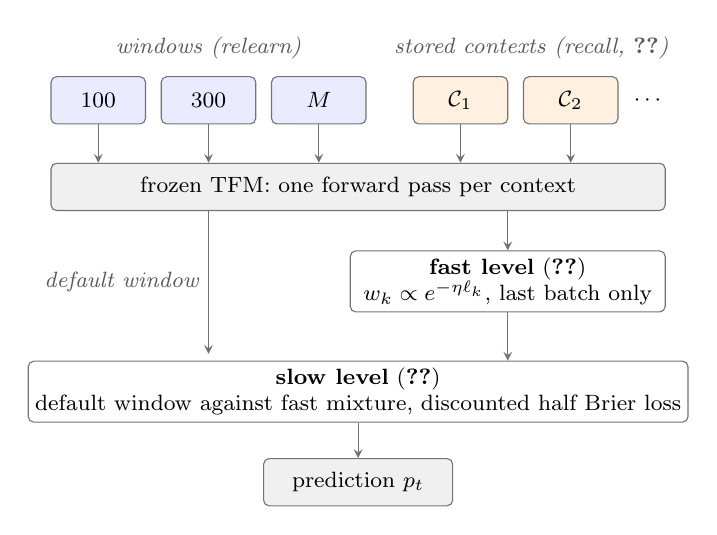
\begin{tikzpicture}[font=\footnotesize, >=stealth,
    box/.style={draw=black!55, rounded corners=2pt, minimum height=6mm, inner sep=2.5pt, align=center, fill=#1},
    box/.default=white,
    lab/.style={font=\footnotesize\itshape, text=black!65}]
  % experts
  \node[box=blue!8, minimum width=12mm] (w1) at (0,0)      {100};
  \node[box=blue!8, minimum width=12mm] (w2) at (1.4,0)    {300};
  \node[box=blue!8, minimum width=12mm] (w3) at (2.8,0)    {$M$};
  \node[box=orange!12, minimum width=12mm] (s1) at (4.6,0) {$\cC_1$};
  \node[box=orange!12, minimum width=12mm] (s2) at (6.0,0) {$\cC_2$};
  \node at (7.0,0) {$\cdots$};
  \node[lab, anchor=south] at (1.4,0.4) {windows (relearn)};
  \node[lab, anchor=south] at (5.5,0.4) {stored contexts (recall, \cref{prop:blind})};
  % frozen TFM
  \node[box=black!6, minimum width=78mm] (tfm) at (3.3,-1.1) {frozen TFM: one forward pass per context};
  \foreach \n in {w1,w2,w3,s1,s2} \draw[->, black!55] (\n.south) -- (\n.south |- tfm.north);
  % fast level (to the right of the default arrow)
  \node[box=white, minimum width=40mm] (fast) at (5.2,-2.3)
       {\textbf{fast level} (\cref{prop:block})\\ $w_k\propto e^{-\eta\ell_k}$, last batch only};
  \draw[->, black!55] (tfm.south -| fast.north) -- (fast.north);
  % slow level
  \node[box=white, minimum width=78mm] (slow) at (3.3,-3.7)
       {\textbf{slow level} (\cref{prop:outer})\\ default window against fast mixture, discounted half Brier loss};
  \draw[->, black!55] (fast.south) -- (fast.south |- slow.north);
  \draw[->, black!55] (1.4,-1.4) -- node[left, lab] {default window} (1.4,-3.22);
  \node[box=black!6, minimum width=24mm] (out) at (3.3,-4.85) {prediction $p_t$};
  \draw[->, black!55] (slow.south) -- (out.north);
\end{tikzpicture}
}
  \caption{\method{} for one batch. Windows and stored contexts are in-context experts of the same frozen TFM. The
  fast level mixes all experts from their losses on the last labelled batch; the slow level mixes the result with the
  default window. Each component is governed by one result of \cref{sec:theory}.}
  \label{fig:method}
\end{figure}

\textbf{Experts.} \emph{Windows} are FIFO contexts of the last 100, 300 and $M$ labelled rows; they relearn fast and
cover concepts that are new or cheap to learn. \emph{Stored concepts} are contexts kept in a pool. Every 500 labelled
rows close a segment $S$. The segment joins the stored expert $\cC_k$ that minimises the estimated recall regret
$\widehat{\Div}_T(S\,|\,\cC_k)=\hat\epsilon_S(\cC_k)-\hat\epsilon_S(S)$ if this is at most $\delta=0.02$, where
$\hat\epsilon_S(S)$ is cross-fitted in two folds because an in-context learner memorises its context; otherwise it
founds a new stored expert (\cref{prop:blind}). A stored expert keeps its last $M$ rows, and the pool holds at most
12 experts (least recently used out).

\textbf{Fast level.} The windows and the stored experts are mixed with the weights \eqref{eq:fast}, $\eta=10$
(\cref{lem:margin,prop:block}).

\textbf{Slow level.} The fast mixture and the $M$-row window are mixed by \eqref{eq:outer-loss}--\eqref{eq:outer}
with $\gamma=0.9$ and $\eta_2=\tfrac12$ (\cref{prop:outer,cor:outer}).


The cost is one TFM call per expert and batch, at most 15, plus three calls when a segment closes. All constants
were set on synthetic development streams; none was tuned on a real stream.

\begin{algorithm}[tb]
\caption{\method{} for one batch $t$}\label{alg:mice}
\begin{algorithmic}[1]
\STATE \textbf{Input:} unlabelled batch $X_t$; labels of batch $t-1$; windows $\mathcal W$; pool $\mathcal P$
\STATE update the windows with batch $t-1$; if 500 new labelled rows: close a segment $S$ and merge it into
       $\argmin_{k\in\mathcal P}\widehat{\Div}_T(S\,|\,\cC_k)$ if the minimum is at most $\delta$, else add $S$ to
       $\mathcal P$
\STATE $\ell_k\leftarrow$ log-loss of expert $k$ on batch $t-1$, for $k\in\mathcal W\cup\mathcal P$
\STATE $p^{\mathrm{fast}}\leftarrow\sum_k w_k\,f_\Theta(\cdot\mid X_t;\cC_k)$ with $w_k\propto e^{-\eta\ell_k}$
\STATE $L_k\leftarrow\gamma L_k+{}$half Brier score of $k\in\{\text{default},\text{fast}\}$ on batch $t-1$
\STATE \textbf{Output:} $v_0\,f_\Theta(\cdot\mid X_t;\cC_{\mathrm{default}})+v_1\,p^{\mathrm{fast}}$ with
       $v_k\propto e^{-\eta_2\gamma L_k}$
\end{algorithmic}
\end{algorithm}

% =====================================================================================================
\section{Experiments}
\label{sec:exp}

The experiments answer four questions. \textbf{RQ1}: does the learning curve predict the value of memory?
\textbf{RQ2}: does \method{} recall, that is, exceed relearning and window ensembles when concepts recur?
\textbf{RQ3}: is \method{} safe and accurate on real streams, where recurrence is weak or absent?
\textbf{RQ4}: what does each component contribute, and do the theoretical conditions hold?

\textbf{Protocol.} Prequential evaluation in batches of $B=100$ rows with labels one batch late; context budget
$M=1000$ for every policy; backbone TabPFN v2 with four ensemble members \citep{hollmann2025tabpfn}, and TabICL
\citep{qu2025tabicl} as a second backbone.

\textbf{In-context baselines}: FIFO; the dual memory (LTM) of
\citet{lourenco2026streams}; DDM-triggered reset \citep{gama2004ddm}; a window ensemble of the three windows of
\method{} without the pool. \textbf{Other stream learners}: Adaptive Random Forest \citep{gomes2017arf}, Streaming
Random Patches \citep{gomes2019srp}, the Hoeffding Adaptive Tree \citep{bifet2009hat}, Leveraging Bagging
\citep{bifet2010levbag}, ADWIN Bagging, Learn++.NSE \citep{elwell2011nse}, and MOOE with trained experts
\citep{zhao2025mooe}, tuned on the development streams over 72 configurations and an extension of its grid
(\cref{app:details}).

\textbf{Streams.} A controlled grid of recurring concepts: mixtures of 5, 30 or 100 Gaussian
centroids whose class assignment is permuted between three concepts, so that $P_X$ is fixed and concepts conflict;
blocks of 500 or 2000 rows; three cycles. Thirty streams from six standard generators (SEA, Stagger, Agrawal, Sine,
RBF, Hyperplane) with recurring concepts. Twenty-nine real streams from 13 sources, the long ones in segments
of 100{,}000 rows: Electricity, seven INSECTS streams \citep{souza2020insects} (one in three segments), Forest
CoverType, PokerHand and Airlines (five segments each), Rialto, NOAA Weather, Spam and Phishing.

\textbf{Pre-registration.} Hypotheses, data and decision rules were written down before each test, and every test
stream was run once. The real streams were opened in five stages (\cref{tab:real}). The first three were also used,
after their one-time evaluation, to develop the slow level. The third held-out set (eight later segments of four
streams) and the grid seeds 20 and 21 were evaluated after the two-level rule was frozen with a step of 10; the step
$\tfrac12$ required by \cref{prop:outer} was added to that analysis before any result was computed. The fourth
held-out set, six further segments that no method had loaded, was then run once with \method{} exactly as defined
in \cref{sec:method} as the registered method (\cref{app:prereg}).


\subsection{RQ1: The Learning Curve Predicts the Value of Memory}
\label{sec:rq1}

We measured the learning curves of the grid concepts, wrote down the gain predicted by \cref{prop:recall}, and only
then ran the streams. On seeds 10 and 11 the fast level alone exceeds reset on all eight streams with 30 or 100
centroids, more for shorter blocks and for harder concepts, as predicted, and the rank correlation between predicted
and observed gain over the six cells is 0.94; the magnitudes agree as well (0.55 versus 0.53 points, 3.0 versus 2.6,
10.4 versus 8.6). On the fresh seeds 20 and 21 with the full two-level method the correlation is 0.83
(\cref{tab:grid,fig:recall}). The six standard generators are the other end of the scale: their learning curves are flat after
about 200 rows, the predicted gain is at most 0.4 points, and the observed gain of \method{} over reset is 0.1 points
on average. Recurring-concept memory cannot be evaluated on the standard generators with a TFM; it needs concepts
that are costly to learn.

\begin{figure}[t]
  \centering
  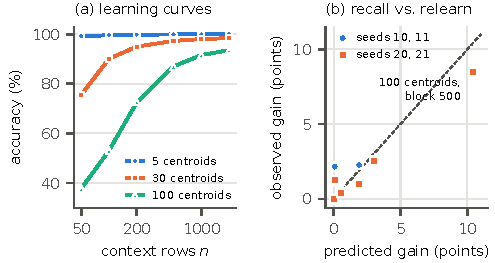
\includegraphics[width=\columnwidth]{fig_recall.pdf}
  \caption{(a) Learning curves of the grid concepts with TabPFN v2, measured before the grid streams were run.
  (b) Gain of memory over reset per grid cell: predicted from these curves by \cref{prop:recall} against observed, for
  the fast level on seeds 10 and 11 and for \method{} on seeds 20 and 21; the dashed line is equality.}
  \label{fig:recall}
\end{figure}

\begin{table}[t]
  \centering
  \caption{Controlled grid, fresh seeds 20 and 21 (accuracy in \%, mean of two streams per cell). Win.: window ensemble; Fast: the
  fast level without the slow level. Pred.: gain over reset predicted by \cref{prop:recall} from learning curves
  measured beforehand; Gain: observed \method{} minus reset, in points.}
  \label{tab:grid}
  \footnotesize
  \setlength{\tabcolsep}{2.2pt}
  \begin{tabular}{rrccccccc}
    \toprule
    Cent. & Block & FIFO & Win. & Reset & Fast & \method{} & Pred. & Gain \\
    \midrule
\rowinput{tab_grid_rows.tex}
    \bottomrule
  \end{tabular}
\end{table}

\begin{table*}[!t]
  \centering
  \caption{Real streams: mean accuracy (\%) per evaluation stage, and the worst difference to FIFO over the streams
  of the stage (points). Every stage was run once when it was opened; the third and fourth held-out sets were opened after the
  two-level rule was frozen. Per-stream results are in \cref{tab:realfull}.}
  \label{tab:real}
  \small
  \setlength{\tabcolsep}{4pt}
  \resizebox{\textwidth}{!}{%
  \begin{tabular}{lccccccc|cccc}
    \toprule
     & & \multicolumn{6}{c|}{Mean accuracy} & \multicolumn{4}{c}{Worst difference to FIFO} \\
    Stage & Streams & FIFO & LTM & Reset & Win.\ ens. & Fast only & \method{} & Reset & Win.\ ens. & Fast only & \method{} \\
    \midrule
\rowinput{tab_real_summary_rows.tex}
    \bottomrule
  \end{tabular}}
\end{table*}

\subsection{RQ2: Recall under Recurring Concepts}
\label{sec:rq2}

On the grid \method{} exceeds reset on all eight streams with 30 or 100 centroids and the window ensemble on all
eight (\cref{tab:grid}): the gain comes from memory, not from faster adaptation. Averaged over the twelve streams it
reaches 86.5 against 84.3 for reset, 81.8 for the window ensemble and 62.4 for FIFO; on the hardest cell the gain
over reset is 8.5 points. The slow level costs 0.4 points here against the fast level alone, the price of the
safeguard. Stream learners that train a model are far behind when a concept must be learned within a block: on seeds
10 and 11, ARF reaches 68.0, SRP 69.7 and the tuned MOOE 78.1, against 83.9 for reset and 86.2 for \method{}. On the
thirty generator streams \method{} matches reset (95.0 against 94.8), and the forgetting of \cref{obs:forget} is
repaired: 0.82--0.89 in the five batches after a recurrence against 0.17--0.51 for FIFO.

\subsection{RQ3: Real Streams}
\label{sec:rq3}


Real streams rarely announce a recurrence, and the experts are close to each other. Here the requirement is
safety first. \Cref{tab:real} shows that every policy that reacts to the last errors pays for it somewhere: reset
loses up to 9.6 points to FIFO (PokerHand) and 1.8 on average, the window ensemble up to 1.4, and the fast level
alone up to 2.3. \method{} loses at most 0.25 points on any of the 29 streams, is above FIFO on 24 of them (+0.57 on
average), and is more accurate than all four in-context baselines on 23. Its largest gains are where the stream
revisits its past, Rialto (+4.7 points over FIFO, with a daily cycle) and the INSECTS streams (+0.2 to +1.9).

\textbf{Confirmatory sets.} On the fourth held-out set all four registered hypotheses hold: \method{} is not below
FIFO or reset on any of the six segments (worst difference to FIFO $-0.01$ points), it is more accurate than all four
in-context baselines on five segments and has the highest mean (85.3 against 85.1 for FIFO, 84.2 for the window
ensemble and 80.9 for reset), and it exceeds its own variant without the pool on all six. The fast level alone is
2.0 and 1.9 points below FIFO on the two PokerHand segments, which the slow level turns into $+0.4$ and $+0.5$;
reset is 9.6 and 8.6 points below. On the third held-out set, \method{} is within 0.08 points of FIFO on every
segment, has the highest mean (85.2 against 84.9 for FIFO) and is the most accurate policy on five of eight
segments; the paired difference to FIFO over batches is $+0.30$ points (block-bootstrap 95\% interval
$[+0.20,+0.40]$), and the registered step of 10 gives the same worst case and five of eight segments.

\textbf{A second seed.} We repeated ten segments with another seed of the backbone, under the same registered
hypotheses. On the fourth held-out set all four hold again (most accurate on five of six segments, never below
FIFO). On four segments of the third held-out set, non-inferiority, safety and the highest mean hold, and \method{}
is the most accurate policy on two of the four segments, where the hypothesis asked for three. Over the ten
segments the difference to FIFO has the same sign under both seeds and changes by at most 0.4 points; its minimum
is $-0.08$ points.

\textbf{Beyond accuracy.} \Cref{tab:metrics} adds the macro-F1 score, the one-vs-rest ROC AUC, the expected
calibration error (ECE) and the half Brier score, computed from the stored predictions of every method. On the real
streams the picture of the accuracy carries over for F1 and the Brier score: \method{} has the highest F1 and a lower
Brier score than every baseline; against FIFO its F1 is higher on 24 of 29 streams ($+0.8$ points on average), its
AUC on 25 and its Brier score lower on 26, and against reset on 25, 28 and 28. The exception is the AUC of the dual
memory: LTM has the highest mean AUC (91.0 against 90.5), all of it from the five PokerHand segments (up to 7.3
points), where its class-balanced long-term buffer keeps rows of the rare classes that a window loses; on the
same segments its accuracy is 2.5 to 3.8 points below \method{}, and on the other 24 streams the AUC of \method{}
is 0.2 points higher in the median. On the grid the step $\eta_2=\tfrac12$ has a price in the quality of the probabilities:
\method{} is 0.2 points below the step of 10 in accuracy but 3.1 points in ECE and 1.2 in the Brier score, because a
small step keeps weight on the default window, which is poorly calibrated under conflicting concepts (ECE 16.7);
its ECE is also above that of reset (7.3), while its Brier score is lower (12.7 against 13.1).
The step that \cref{prop:outer} covers is thus the conservative choice: it buys the guarantee with calibration in the
recall regime.

\begin{table*}[!t]
  \centering
  \caption{Metrics beyond accuracy (\%, mean over streams): macro-F1, one-vs-rest ROC AUC, expected calibration error
  (15 bins) and half Brier score, on the 29 real streams and the 24 grid streams. Computed from stored predictions;
  the best value per column is in bold.}
  \label{tab:metrics}
  \small
  \setlength{\tabcolsep}{5pt}
  \begin{tabular}{lccccc|ccccc}
    \toprule
     & \multicolumn{5}{c|}{Real streams} & \multicolumn{5}{c}{Controlled grid} \\
    Method & Acc.\ $\uparrow$ & F1 $\uparrow$ & AUC $\uparrow$ & ECE $\downarrow$ & Brier $\downarrow$
           & Acc.\ $\uparrow$ & F1 $\uparrow$ & AUC $\uparrow$ & ECE $\downarrow$ & Brier $\downarrow$ \\
    \midrule
\rowinput{tab_metrics_rows.tex}
    \bottomrule
  \end{tabular}
\end{table*}

\textbf{Other learners and a second backbone.} On all 29 streams, the best trained
stream learner per stream (seven learners, MOOE in two configurations) is below \method{} on 28 and below FIFO on
23; the exception is one Airlines segment, where Streaming Random Patches is 0.3 points above \method{}. On
CoverType and PokerHand the trained learners are 4 to 19 points behind. With TabICL as the backbone and no constant changed, \method{} is the most accurate policy on all four streams of the
first held-out set (84.0 on average against 83.4 for FIFO and 83.5 for the window ensemble), and in registered
tests on four segments of the third held-out set and on all six of the fourth, the four hypotheses of the kind
above hold: on the fourth set \method{} is the most accurate policy on six of six segments (85.2 on average against
84.7 for FIFO, 84.2 for the window ensemble and 81.3 for reset), and over the ten segments it is at most 0.02 points
below FIFO.

\subsection{RQ4: Components and Conditions}
\label{sec:ablation}

\textbf{Windows and pool.} Removing the pool, so that the two levels mix the three windows only, lowers accuracy on
every one of the 24 grid streams (by 5.6 points on average) and on 28 of the 29 real streams (by 0.35 points on
average, 2.1 on Rialto and 1.5 on a PokerHand segment): memory, not the choice of a window, carries the gain, on real
streams as well. Removing the two short windows instead lowers the generator streams from 95.0 to 93.6 and the grid
from 86.4 to 81.8 and leaves the real streams within 0.2 points on average; the pool forms exactly as many stored
experts as a generator stream has concepts.

\textbf{Slow level.} It leaves the recall regime almost
unchanged (grid: 86.5 against 86.9 for the fast level alone) and removes the losses on real streams (worst case
$-0.25$ against $-2.3$; \cref{tab:real}). With the log-loss in place of the half Brier score, one grid stream falls
from 86.4 to 74.9: after a switch the fast mixture is confidently wrong for one batch, and an unbounded loss lets
that batch outweigh the next ten.

\textbf{Discrepancy.} On 144 pairs of grid segments, the recall regret and the
excess-risk discrepancy separate ``different concept'' from ``same concept'' with AUROC 1.00, and the R-divergence
estimate with 0.85 (0.42 on the hardest cell), as \cref{prop:blind} predicts; on pairs of the same concept the
estimated excess is negative, down to $-0.2$ for 100 centroids, the pooling gain.

\textbf{Margin.} On the grid the
leading expert holds weight 1.000 from the second batch of a recurring block, with a gap of 0.8--8.0 nats to the
runner-up, so $(K-1)e^{-\eta g}<0.005$ in \cref{prop:block}; on the real streams the median gap is 0.008--0.012
nats, the regime for which the slow level is built.

\textbf{Regret.} Over 33 development streams the largest
discounted regret of the slow level is 0.15 against the window and 0.35 against the fast mixture, within the bound
of 1.39; on adversarial sequences the bound holds at $\eta_2=\tfrac12$ and fails for steps of 2 and 10
(\cref{app:details}).

% =====================================================================================================
\section{Related Work}
\label{sec:related}

\textbf{Concept drift and recurring concepts.} Drift detection and adaptation are surveyed by
\citet{gama2014survey} and \citet{lu2019learning}. Recurring concepts are handled by storing past models and
reusing them, selected by statistical tests \citep{goncalves2013rcd}, by meta-learners of each model's domain
\citep{gama2014recurrent} or by weighted ensembles of batch learners \citep{elwell2011nse}. MOOE
\citep{zhao2025mooe} combines offline experts of past intervals with an online expert under a meta expert with
regret guarantees; \method{} keeps its decomposition and replaces trained experts by stored contexts, the
cumulative meta expert by two time scales, and the generic regret by a quantity measured from the learning curve.
\textbf{Model-oriented discrepancy.} R-divergence \citep{zhao2023rdiv} and I-Div \citep{zhao2024idiv} measure
distribution discrepancy through a learned hypothesis; we identify the blind spot of the former under conflicting
concepts and use an excess-risk form to decide which contexts to pool. \textbf{TFMs on streams.}
\citet{lourenco2026streams} show that a TFM with a short- and long-term FIFO memory outperforms incremental
ensembles; Drift-Resilient TabPFN \citep{helli2024drift} retrains the prior to extrapolate temporal trends. Neither
models recurrence. Concept drift has likewise been redefined for other new model families, such as multi-modal
large language models \citep{yang2025adapting,yang2026turning}. \textbf{Online aggregation.} Exponential weights
with exp-concave losses and their logarithmic regret are classical \citep{cesabianchi2006prediction,hazan2007log};
\cref{prop:outer} is their discounted, any-time form for two in-context experts.

% =====================================================================================================
\section{Conclusion}
\label{sec:conclusion}

For an in-context learner, memory of a past concept is free to store and free to recall, and its value is the area
between the learning curve and the accuracy of the stored context. \method{} turns this into a method with one
component per result: an excess-risk discrepancy decides which contexts share a concept, a fast meta expert
identifies a recurring concept in one batch, and a slow meta expert guarantees, at any time and for any stream,
that following it costs little against the plain window. When concepts recur and are costly to learn, \method{}
exceeds reset detection, window ensembles and trained experts by a wide margin; on 29 real streams it is the most
accurate in-context policy on 23 and never more than 0.25 points below a sliding window, where reset detection
loses up to 9.6 points.

\textbf{Limitations.} The gains on real streams other than Rialto are below two points; the claim there is safety
with a small average gain, and the large gains are for recurring concepts with steep learning curves.
The confirmatory real segments come from three streams whose earlier segments were used in development; ten
segments were repeated with a second seed and the others have one run. \Cref{prop:outer} bounds the half Brier score rather than the accuracy, its step costs calibration when
concepts recur (\cref{tab:metrics}), and
\cref{prop:blind} holds under \cref{ass:ppd}, and \cref{prop:recall} under \cref{ass:margin}. \method{} calls the TFM once per
expert, 5--18 times the time of a single context in our runs.

\bibliography{refs}
\bibliographystyle{icml2026}

% =====================================================================================================
\newpage
\appendix
\crefalias{section}{appendix}
\onecolumn

\section{Proofs}
\label{app:proofs}

\subsection{Proof of \texorpdfstring{\cref{prop:blind}}{Proposition 1}}

\begin{proof}
For the log-loss and any conditional $h$,
\[
  \epsilon_P(h)=\E_{P_X}\bigl[H(p_\vx)+\KL(p_\vx\|h_\vx)\bigr],
\]
so that $\epsilon_P(h_P)=\E_{P_X}H(p_\vx)$ and $\epsilon_P(h_U)-\epsilon_P(h_P)=\E_{P_X}\KL(p_\vx\|u_\vx)$, and likewise
for $Q$.

\emph{(i)} By the chain rule, $\KL(P\|U)=\KL(P_X\|U_X)+\E_{P_X}\KL(p_\vx\|u_\vx)$, and the same holds for $Q$.
Averaging the two identities gives
\[
  \mathrm{JS}(P,Q)=\mathrm{JS}(P_X,Q_X)+\Div_E(P,Q),
\]
and $\Div_E\ge0$ as a mean of KL terms. If $P_X=Q_X$, then $\alpha\equiv\tfrac12$, $u_\vx=\tfrac12(p_\vx+q_\vx)$ and
$\Div_E=\E_\vx\mathrm{JS}(p_\vx,q_\vx)$, which vanishes if and only if $p_\vx=q_\vx$ almost surely.

\emph{(ii)} By the display above,
\[
  \Div_R(P\|Q)=\Bigl|\E_{P_X}\bigl[H(p_\vx)+\KL(p_\vx\|u_\vx)\bigr]-\E_{Q_X}\bigl[H(q_\vx)+\KL(q_\vx\|u_\vx)\bigr]\Bigr| .
\]
Deterministic concepts have $H(p_\vx)=H(q_\vx)=0$, and $u_\vx$ puts mass $\tfrac12$ on each of $g_P(\vx)$ and
$g_Q(\vx)$ where they differ and mass $1$ where they agree. Hence
$\KL(p_\vx\|u_\vx)=\KL(q_\vx\|u_\vx)=\ln2\cdot\mathbf 1[g_P(\vx)\neq g_Q(\vx)]$; with $P_X=Q_X$ the two expectations
cancel, and $\Div_E=\rho\ln2$.

\emph{(iii)} Under the 0-1 loss, with ties of $u_\vx$ broken independently of the source of the query, the prediction
of $h_U$ at a disagreeing $\vx$ is $g_P(\vx)$ or $g_Q(\vx)$ with probability $\tfrac12$ each. Each risk is therefore
$\rho/2$ and $\Div_R=0$. The predictor $h_P$ errs on $Q$ exactly where the concepts disagree and $h_Q$ nowhere, so
$\Div_T(Q\,|\,P)=\rho$.
\end{proof}

\subsection{Proofs of \texorpdfstring{\cref{lem:margin,prop:block}}{Lemma 1 and Proposition 2}}

\begin{proof}[Proof of \cref{lem:margin}]
\emph{(i)} By \cref{ass:margin},
\[
  w_{k^\star}=\Bigl(1+\sum_{k\ne k^\star}e^{-\eta(\ell_k-\ell_{k^\star})}\Bigr)^{-1}\ge\bigl(1+(K-1)e^{-\eta g}\bigr)^{-1}=e^{-\kappa}.
\]
\emph{(ii)} For a row with label $y$ and expert predictions $p_k$,
\[
  -\ln\sum_kw_kp_k(y)\;\le\;-\ln\bigl(w_{k^\star}p_{k^\star}(y)\bigr)\;\le\;-\ln p_{k^\star}(y)+\kappa .
\]
\emph{(iii)} For two classes $y_1,y_2$,
\[
  \sum_kw_k\bigl(p_k(y_1)-p_k(y_2)\bigr)\;\ge\;w_{k^\star}\bigl(p_{k^\star}(y_1)-p_{k^\star}(y_2)\bigr)-(1-w_{k^\star}),
\]
which is positive when the gap of expert $k^\star$ exceeds $(1-w_{k^\star})/w_{k^\star}\le e^{\kappa}-1$.
\end{proof}

\begin{proof}[Proof of \cref{prop:block}]
The first batch of the block is predicted with weights from a batch of the previous concept; its per-row regret is
at most $c$. Every later batch is predicted with weights from a labelled batch of the block, on which $k^\star$
leads by $g$, so \cref{lem:margin}(ii) bounds its per-row regret by
$\ln\bigl(1+(K-1)e^{-\eta g}\bigr)\le(K-1)e^{-\eta g}$. Summing over the $J-1$ later batches gives the claim.
\end{proof}

\subsection{Proofs of \texorpdfstring{\cref{prop:recall,cor:flat}}{Theorem 1 and Corollary 1}}

\begin{proof}[Proof of \cref{prop:recall}]
Both learners lose the first batch of the block, whose labels have not arrived. Before batch $j+1$
($j=1,\dots,J-1$) the relearning context holds $\min(jB,M)$ rows of the block, so its expected accuracy is
$a_k(\min(jB,M))$; the stored expert has expected accuracy $a_k(n_c)$. By \cref{lem:margin}(iii) the mixture
predicts as the better of the two, so its expected accuracy is the larger of the two values, and the difference to
relearning is the positive part in \eqref{eq:area}. Averaging over the $J$ batches gives the claim.
\end{proof}

\begin{proof}[Proof of \cref{cor:flat}]
On the first visit the pool holds no expert of the concept, so the mixture and the relearning learner use the same
rows. Since $a_k$ is non-decreasing and $n_c\le M$, every term of \eqref{eq:area} is at most $a_k(M)-a_k(B)$, which
is zero for a flat curve, and the terms with $jB\ge M$ vanish. At most $M/B$ of the $J=L/B$ terms are non-zero,
which gives the bound.
\end{proof}

\subsection{Proofs of \texorpdfstring{\cref{prop:outer,cor:outer}}{Theorem 2 and Corollary 2}}

\begin{proof}[Proof of \cref{prop:outer}]
\emph{Exp-concavity.} The half Brier score $\ell(p)=\tfrac12\lVert p-e_y\rVert^2$ has gradient $p-e_y$ and Hessian
$I$, and $\lVert p-e_y\rVert^2\le2$ on the simplex. Hence
$\nabla^2\ell\succeq\eta_2\,\nabla\ell\nabla\ell^{\top}$ for $\eta_2\le\tfrac12$, that is, $\ell$ is
$\eta_2$-exp-concave. The mean over the rows of a batch is $\eta_2$-exp-concave as well: its Hessian is the mean
Hessian, and $\tfrac1n\sum_ig_ig_i^\top\succeq\bar g\bar g^\top$ for the row gradients $g_i$ with mean $\bar g$.
Consequently
\begin{equation}\label{eq:expconcave}
  e^{-\eta_2\ell_t(p_t)}\;\ge\;\sum_kv_{t,k}\,e^{-\eta_2\ell_{t,k}} .
\end{equation}
\emph{Potential.} Let $W_t=\sum_ke^{-\eta_2L_{t,k}}$, so that $W_0=K$. By \eqref{eq:outer-loss} and
\eqref{eq:outer-weight},
\[
  W_t=\Bigl(\sum_ke^{-\eta_2\gamma L_{t-1,k}}\Bigr)\sum_kv_{t,k}\,e^{-\eta_2\ell_{t,k}} .
\]
By the power-mean inequality, $\sum_kx_k^{\gamma}\le K^{1-\gamma}\bigl(\sum_kx_k\bigr)^{\gamma}$ for $x_k\ge0$ and
$\gamma\in(0,1]$; with $x_k=e^{-\eta_2L_{t-1,k}}$ and \eqref{eq:expconcave},
\[
  \ln W_t\;\le\;(1-\gamma)\ln K+\gamma\ln W_{t-1}-\eta_2\,\ell_t(p_t).
\]
\emph{Unrolling.} Since $(1-\gamma)\sum_{t\le T}\gamma^{T-t}+\gamma^{T}=1$,
\[
  \ln W_T\;\le\;\ln K-\eta_2\sum_{t=1}^{T}\gamma^{T-t}\ell_t(p_t).
\]
On the other hand $\ln W_T\ge-\eta_2L_{T,k}=-\eta_2\sum_{t=1}^{T}\gamma^{T-t}\ell_{t,k}$ for every $k$. Combining the
two inequalities gives \eqref{eq:outer-bound}.
\end{proof}

\begin{proof}[Proof of \cref{cor:outer}]
Insert $K=2$ and $\eta_2=\tfrac12$ into \eqref{eq:outer-bound}; the discounted number of batches is
$\sum_{t\le T}\gamma^{T-t}\le1/(1-\gamma)$.
\end{proof}

\section{Pre-Registration Record}
\label{app:prereg}

All hypotheses below were written to the experiment log before the corresponding streams were run, and every test
stream was run once; interrupted runs were resumed from their checkpoints without rerunning a finished cell.

\textbf{Grid, seeds 10 and 11} (fast level alone). Hypotheses: gain over reset positive on all eight streams with 30
or 100 centroids, larger for shorter blocks and for more centroids; Spearman correlation between predicted and
observed gain at least 0.8; the window ensemble below the method on these eight streams. All held (correlation
0.94). An incidental expectation of no gain with 5 centroids was missed on one stream, where the reset baseline
detected late.

\textbf{Generator streams, seeds 10--14, and five real development streams.} Non-inferiority to reset on the
generator streams ($+0.50$ points, 25 of 30 positive) and on each real stream held, as did the replication of
\cref{obs:forget}. An exploratory expectation that the INSECTS stream with re-occurring drift would gain most was not
met (it ranked second).

\textbf{First held-out set} (four streams; fast level alone). Non-inferiority to reset on every stream and highest
mean accuracy held; the method was the most accurate on three of four streams. A replication with TabICL held as
well.

\textbf{Second held-out set} (six streams; fast level alone). Non-inferiority to reset held. The hypothesis that the
fast level alone would be the most accurate method on at least four of six streams was \emph{not} met (one of six),
and on PokerHand it was 2.3 points below FIFO. This result motivated the slow level; all real streams seen so far
count as development data from here on.

\textbf{Third held-out set} (eight segments; two-level rule frozen). Two candidates for the slow level were
registered before any result existed: the log-loss with step 1, and the half Brier score with step 10, added after
the log-loss failed on a cached synthetic test stream. For both, non-inferiority to FIFO and reset (tolerance 0.5
points) and to the fast level alone held on every segment, and the mean was the highest. ``Most accurate on at least
five of eight segments'' held for the half Brier score (five) and not for the log-loss (four). The step
$\eta_2=\tfrac12$ with tempered weights, the method of this paper, was added to the analysis after the baselines of
three segments were visible and before any result of a two-level rule was computed; it was not part of the
registered hypotheses. It gives five of eight segments and the highest mean.

\textbf{Fourth held-out set} (six segments: the next 200{,}000 rows each of Airlines, PokerHand and CoverType; method of
\cref{sec:method} frozen). Registered hypotheses: on every segment not more than 0.5 points below the better of FIFO
and reset; above all four in-context baselines on at least four of six segments, with the highest mean; on every
segment not more than 0.3 points below FIFO; above the variant without the pool on at least four of six segments.
All held (five of six segments; worst difference to FIFO $-0.01$ points; six of six against the variant without the
pool).

\textbf{Second backbone and second seed.} With the method of \cref{sec:method} frozen and the same four hypotheses
(``at least three of four'' for sets of four segments): TabICL on four segments of the third held-out set and on the
six segments of the fourth, all held; a second seed of TabPFN on the same four segments, three held and ``most accurate on at least three of four
segments'' did not (two); a second seed on the six segments of the fourth held-out set, all held.

\textbf{Grid, seeds 20 and 21} (half Brier score, step 10). Mean difference to the fast level alone at least $-0.5$
points ($-0.14$), above reset on all eight streams with 30 or 100 centroids, and within one point of reset with 5
centroids: all held. The step $\tfrac12$ is 0.23 points lower on average and satisfies the same three statements.

\section{Experimental Details and Full Results}
\label{app:details}

\textbf{Streams.} The grid and generator streams are produced by \texttt{code/grid\_streams.py} and
\texttt{code/streams.py}; generator streams have blocks of 2000 rows and three cycles over three or four concepts.
Real streams with more than 100{,}000 rows are cut into segments of 100{,}000 (CoverType and one INSECTS stream:
150{,}000 for the first segment). The second held-out set consists of all streams of a public collection of drift
data sets that have at least 5000 rows, at most ten classes and had not been used before.
\textbf{Baselines.} LTM follows Algorithm~1 of \citet{lourenco2026streams} with a short-term share of 0.75. MOOE
follows the original algorithm with linear experts on random Fourier features, generalised to several classes; it
was tuned on the five development streams over feature type, interval length, step size and regularisation (72
configurations), and its grid was extended twice because the optimum lay on the boundary; the best configuration of
every round is evaluated. The incremental learners use the default settings of \texttt{river} \citep{montiel2021river}
with ten base models and the same batch protocol.
\textbf{Regret under adversarial sequences.} With synthetic expert predictions and labels chosen to hurt the mixture
or the current leader ($K\in\{2,5\}$, $\gamma\in\{0.5,0.9,0.99,1\}$, 400 rounds), the discounted regret at
$\eta_2=\tfrac12$ stays below $\ln K/\eta_2$ in every configuration (at most 0.67 for $K=2$), exceeds it at
$\eta_2=2$ for $\gamma\ge0.9$, and reaches 4.4 at $\eta_2=10$, $\gamma=0.9$.

\begin{table}[h]
  \centering
  \caption{Real streams: accuracy (\%) per stream. Fast only: the fast level without the slow level; $\eta_2=10$: the
  pre-registered step; Trained: the best trained stream learner per stream;
  $\Delta$: \method{} minus FIFO in points.}
  \label{tab:realfull}
  \small
  \begin{tabular}{lccccccccc}
    \toprule
    Stream & FIFO & LTM & Reset & Win.\ ens. & Fast only & $\eta_2=10$ & \method{} & Trained & $\Delta$ \\
    \midrule
\rowinput{tab_real_rows.tex}
    \bottomrule
  \end{tabular}
\end{table}

\end{document}
